\section{Repository}
\label{repository}
In questa sezione sono definiti gli strumenti utilizzati per la condivisione e il versionamento dei vari file.
\\Per la gestione della documentazione e dei file di codifica sono stati creati due repository\glossario{} distinti. 
I repository\glossario{} sono privati e quindi accessibili solo ai membri del gruppo \authorName.
\\I repository\glossario{} sono ospitati dal servizio GitHub\glossario{}, il quale utilizza il sistema di versionamento Git\glossario{}.

\subsection{Repository della documentazione}
\label{rdocumentazione}
L'URL del repository\glossario{} della documentazione è: \url{https://github.com/nicolobissacco/7MonkeysDoc}.
\\All'interno di questo repository\glossario{} verranno memorizzati tutti i file necessari alla generazione dei documenti. Di seguito verrà descritta sinteticamente l'organizzazione interna del filesystem.

\begin{figure}[h!]
\centering
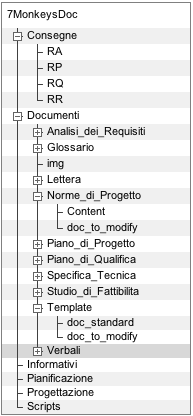
\includegraphics[height=7cm]{./content/Immagini/Filesystem.png}
\caption{Organizzazione file system del repository dei documenti.}
\label{filesystem}
\end{figure}

\begin{itemize}
\item\textbf{Consegne:} contiene tutti i documenti in formato \verb!PDF!\glossario{} consegnati nelle varie revisioni. I file sono raggruppati in sotto cartelle denominate con l'acronimo della revisione a cui fanno riferimento. La struttura delle sottocartelle sarà la seguente:
\begin{itemize}
\item\textbf{RR:} Revisione dei Requisiti;
\item\textbf{RP:} Revisione di Progettazione;
\item\textbf{RQ:} Revisione di Qualifica;
\item\textbf{RA:} Revisione di Accettazione.
\end{itemize}

\item\textbf{Documenti:} è la cartella contenente i sorgenti di tutti i documenti, sia in stato di redazione, sia completati. Il suo contenuto è organizzato nel seguente modo:
\begin{itemize}
\item\textbf{Nome\_del\_Documento:} ogni documento in fase di redazione dovrà avere la propria cartella, denominata con lo stesso nome del documento (vedi \ref{filesystem}). Se il documento necessità di immagini, esse dovranno essere salvate in una sottocartella denominata \lq\lq{}Immagini\rq\rq{};
\item \textbf{Template:} contiene i template \LaTeX{} comuni a tutti i documenti necessari per la loro compilazione. In particolare, in essi vengono definiti gli stili delle pagine, il frontespizio e i vari comandi creati per la stesura;
\item \textbf{Verbali:} contiene i verbali redatti dal gruppo durante lo svolgimento del progetto. Per ogni documento verrà creata una sottocartella apposita, contenente i file necessari.
\end{itemize}

\item\textbf{Informativi:} contiene dei files informativi; per esempio è presente una procedura per la creazione di un nuovo documento e un file contenente la lista di tutti i comandi \LaTeX utilizzati nei files di compilazione;

\item\textbf{Pianificazione:} contiene tutti i grafici Gantt\glossario{} utilizzati nella pianificazione delle attività e nella gestione delle risorse;

\item\textbf{Progettazione:} contiene tutti i diagrammi UML\glossario{} utilizzati durante la progettazione del software;
\item\textbf{Scripts:} contiene gli scripts utilizzati per automatizzare alcune procedure; per esempio la compilazione dei documenti per una consegna.
\end{itemize}

\subsection{Repository del codice}
\label{repocodice}
L'URL del repository\glossario{} del codice è: \url{https://github.com/nicolobissacco/7MonkeysCode}.
La struttura del repository\glossario{} verrà decisa durante la fase di \emph{Progettazione di Dettaglio}.